\documentclass[fontsize=55pt,  paper=a2, pagesize]{scrartcl}
% page number suppressed 
\pagenumbering{gobble}
\usepackage{graphicx}
% see https://tex.stackexchange.com/questions/614621/tabularray-and-rgb-xcolor-option
\usepackage{xcolor}
\usepackage{tabularray}
\UseTblrLibrary{siunitx}
\UseTblrLibrary{booktabs}
\usepackage{setspace}

\definecolor{pepgray}{HTML}{565656}
\definecolor{peporange}{HTML}{FFB137}
\colorlet{strokeColor}{white}
\colorlet{fillColor}{pepgray}
\colorlet{textColor}{black}

% set font almost like poster
\usepackage{fontspec}
\newfontfamily\bodyfont[]{Fira Sans}
\newfontfamily\thinfont[]{Fira Sans Light}
\newfontfamily\headingfont[]{Fira Sans Bold}
\newfontfamily\emphfont[]{Fira Sans Italic}
\newfontfamily\monofont[]{Fira Mono}
\renewcommand{\em}{\emphfont\color{textcolor}}

\setmainfont{Merriweather Regular}

% get control over borders
\usepackage[ a2paper, margin=1cm, %
            ignoreall, noheadfoot, nomarginpar, %top=-1in %
            %showframe %
            ]{geometry}
            % use tikz
\usepackage{tikz}
\usetikzlibrary{calc}
\usetikzlibrary{svg.path}

% Hyperlinks
\usepackage[
  allbordercolors = pepgray,
  unicode,        % Unicode in PDF-Attributen erlauben
  pdfusetitle,    % Titel, Autoren und Datum als PDF-Attribute
  pdfcreator={},  % ┐ PDF-Attribute säubern
  pdfproducer={}, % ┘
]{hyperref}

\begin{document}
\thispagestyle{empty}

% set new length unit
\newlength\ulen
\setlength\ulen{1cm}
\setlength\parindent{0cm}

% use tikzpicture environment to move objects around 
% options: use tikz as overlay, shift that (0,0) os upper left corner and set the default length units
\begin{tikzpicture}[remember picture, overlay, shift=(current page.north west), x=\ulen, y=\ulen]

  \begin{scope}[shift={($(current page.north)+(0, -3)$)}]
    \node[anchor=north,text width=25\ulen, color=textColor] (pep) at (5.5\ulen, 0) {%
    {\Large\headingfont Bachelorkolloquien}\\
    {\setstretch{0.7}
    {\headingfont im \monthname}\\[1ex]
    \thinfont
    von PeP et al.~e.\kern-0.1333em V\kern-0.1333em.\par
    }
    };

    \begin{scope}[anchor=east, scale=5, shift={($(pep.west)+(-1, 0)$)}]
      \fill[color=fillColor] (0, 0) circle[radius=1\ulen];
      \draw[
        color=strokeColor,
        line width=1pt,
        smooth,
        yscale=0.9,
        xscale=0.57,
        xshift=-0.5cm,
        domain=-1.20:2.25,
        samples=200,
      ] plot (\x, {exp(-\x * \x) * cos(10 * deg(\x))});
    \end{scope}
  \end{scope}

  \node (info) at ($(current page.north)+(0, -13)$)%
  [anchor=north,color=textColor,text width=35\ulen,font=\fontsize{36pt}{42pt}\selectfont,align=justify]%
  {
    Du möchtest nächstes Semester deine Bachelorarbeit schreiben, weißt aber noch nicht zu welchem Thema? Dann ist das Bachelor-Kolloquium genau richtig für dich.\\
    Das Kolloquium findet {\color{peporange} montags von 12:15 Uhr bis ca. 13:15 Uhr im AV-Raum (P2-E0-414)} des Physik Gebäudes statt.
  };
  \node[anchor=north, color=textColor] at (info.south)
  {
    \centering
    \fontsize{42pt}{42pt}\selectfont
    \speakers
  };

  \begin{scope}[shift={($(current page.west)+(33.5, -16)$)}, xscale=-9, yscale=9]
    % \fill[color=fillColor] (0, 0) circle[radius=1\ulen];
    \fill[
      color=fillColor,
      line width=1pt,
      smooth,
      yscale=0.9,
      xscale=0.57,
      xshift=-0.5cm,
      domain=-1.20:2.25,
      samples=200,
    ] plot (\x, {.5*exp(-(\x+10) * (\x+10)) * cos(10 * deg(\x))+.5*exp(-\x * \x) * cos(10 * deg(\x))}) -- ++(20, 0) -- ++(0, -20) -- ++(-40, 0) -- ++(0, 20)  -- cycle;
  \end{scope}
  \node[anchor=south, color=white, text width=\linewidth, align=center] (link) at ($(current page.south)+(0, .5)$)
  {
    \colorbox{white}{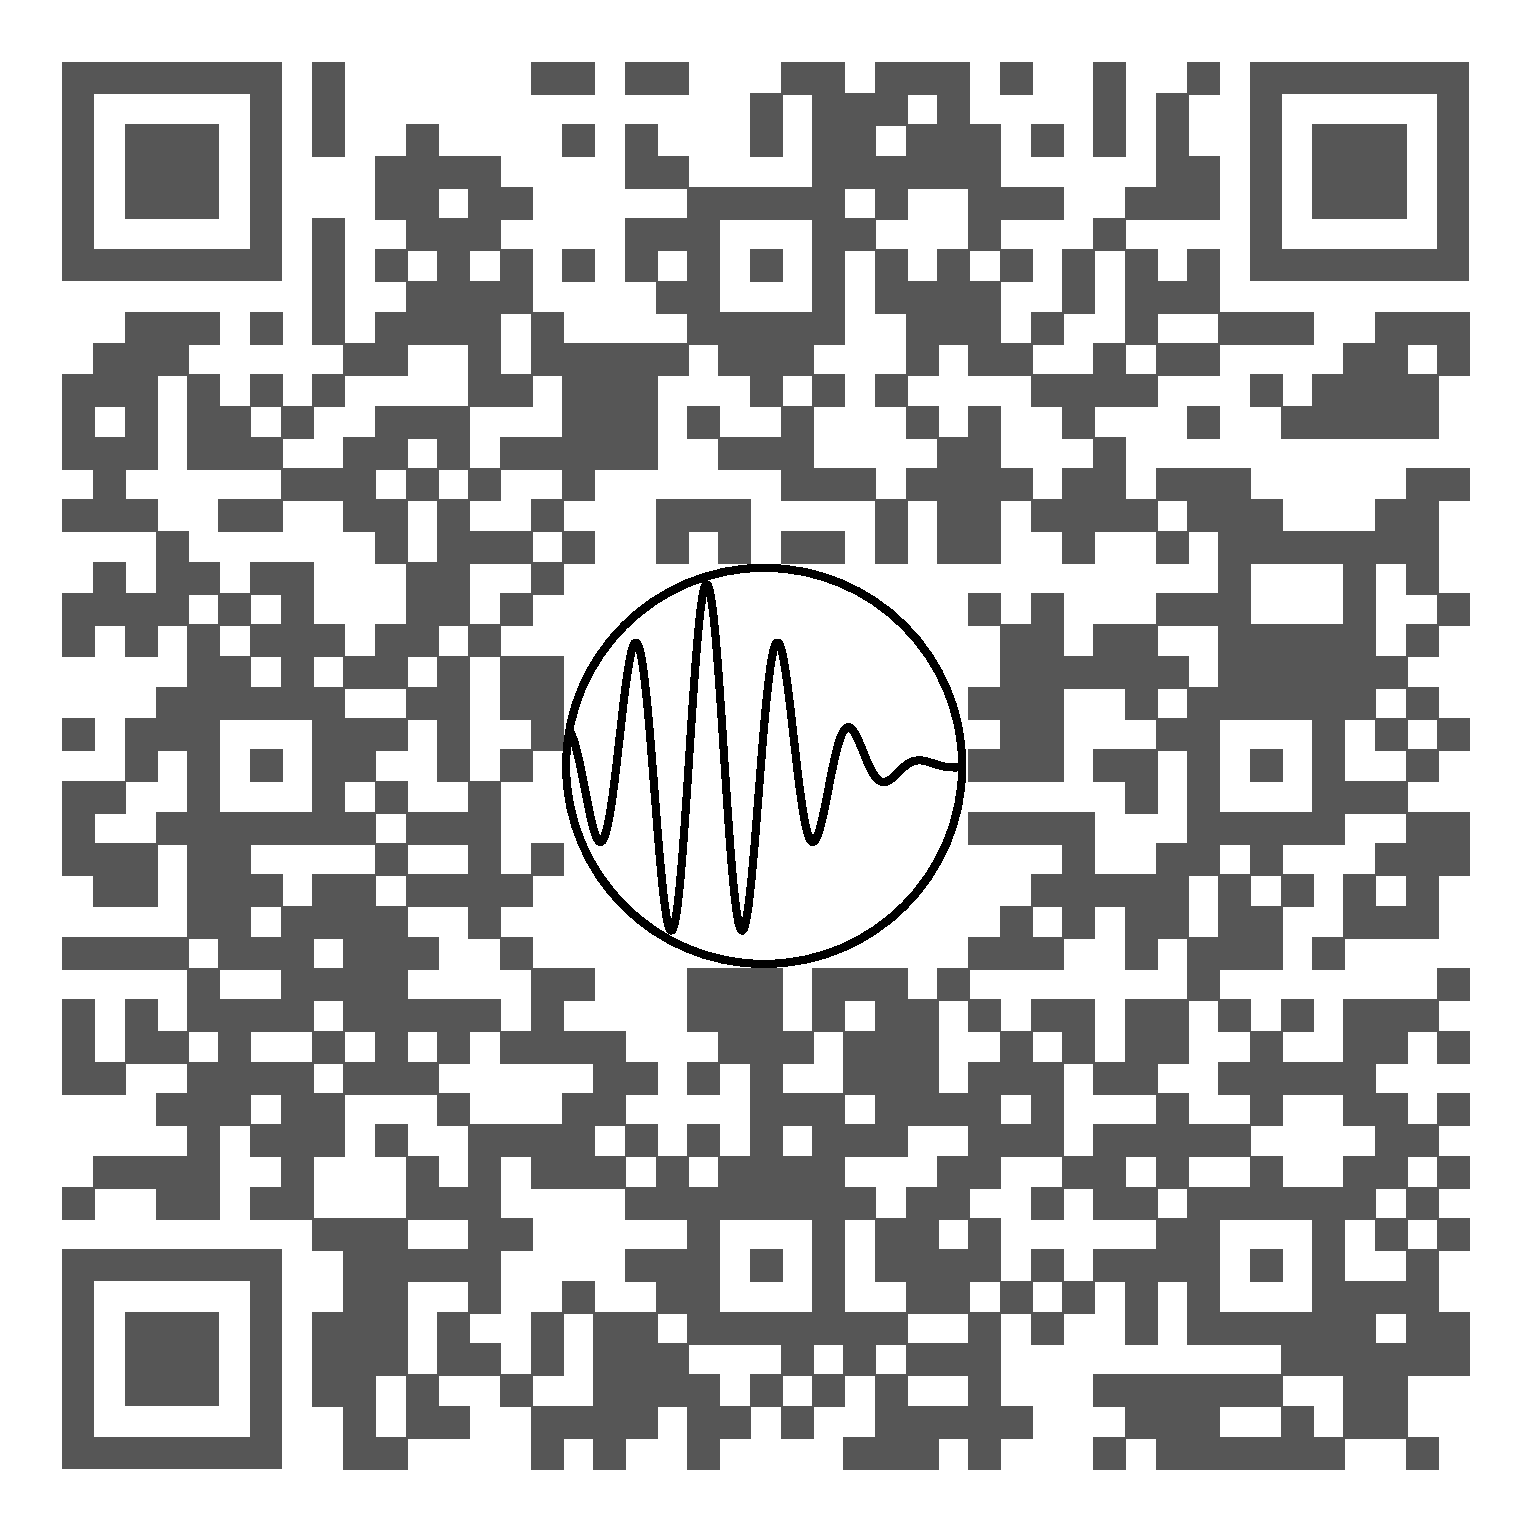
\includegraphics[width=.2\linewidth]{qr.pdf}}
    \\[-.5ex] \href{https://pep-dortmund.de/vereinsleben/bachelorkolloquium.html}{\scriptsize\monofont \mbox{pep-dortmund.de/vereinsleben/bachelorkolloquium.html}}};
\end{tikzpicture}

\end{document}
